\documentclass[10pt,aspectratio=169]{beamer}
\usetheme[progressbar=frametitle,numbering=fraction,block=fill]{metropolis}
\usepackage[T1]{fontenc}
\usepackage[utf8]{inputenc}
\usepackage{amsmath,amssymb,bm}
\usepackage{siunitx}
\sisetup{per-mode=symbol}
\usepackage{booktabs}
\usepackage{graphicx}
\usepackage{tikz}
\usetikzlibrary{positioning,arrows.meta}
\usepackage{xcolor}
\usepackage{listings}
\graphicspath{{../figures/}}

\definecolor{sfblue}{HTML}{2A78D6}
\definecolor{sforange}{HTML}{EB6834}
\definecolor{sfgray}{HTML}{898781}
\definecolor{sfink}{HTML}{23373B}
\setbeamercolor{progress bar}{fg=sfblue}
\setbeamercolor{title separator}{fg=sfblue}
\setbeamercolor{alerted text}{fg=sforange}
\setbeamercolor{frametitle}{bg=sfink}
\lstset{basicstyle=\ttfamily\scriptsize,columns=fullflexible,keepspaces=true,breaklines=true}

\newcommand{\dv}{\Delta v}
\newcommand{\vinf}{v_\infty}
\newcommand{\code}[1]{\texttt{#1}}

\title{A Patched-Conic Mission Analysis Tool}
\subtitle{Lunar \& interplanetary design --- approach, validation, limitations}
\author{MECE 4305 Mechanics \& Thermodynamics of Propulsion --- Week 10}
\institute{Columbia University, Fall 2026 \quad\textbullet\quad \code{mission\_analysis} (\code{sfmission}) v0.1}
\date{9 November 2026}

\begin{document}
\maketitle

%------------------------------------------------------------------
\begin{frame}{Why: the first four steps of the design roadmap}
\small
\begin{columns}[T]
\begin{column}{0.55\textwidth}
\begin{enumerate}
\item \textbf{Mission definition} --- target, dates, orbits
\item \textbf{Required $\dv$} --- launch, injection, flybys, capture, landing
\item \textbf{Propellant mass fraction $\rightarrow$ required $I_{sp}$}
\item \textbf{Staging / architecture}
\item[5--10.] thrust, thrust chamber, $\dot m$, $V_e$, $p_c$, $M_e$, $A_e$, feed system, iterate \hfill \textcolor{sfgray}{(Weeks 11--12)}
\end{enumerate}
\medskip
The tool computes steps 1--4 and hands a \code{DeltaVBudget} with propellant masses and required $I_{sp}$ to the engine-design steps.
\end{column}
\begin{column}{0.43\textwidth}
\begin{block}{Three uses}
\begin{itemize}
\item Week-10 lecture instrument (live porkchop of the window opening \emph{this month})
\item HW~1 reference solution and the first module of each team's project model
\item Preliminary design tool exposed to agents via MCP
\end{itemize}
\end{block}
\end{column}
\end{columns}
\end{frame}

%------------------------------------------------------------------
\begin{frame}{What it computes}
\footnotesize
\begin{tabular}{p{0.22\textwidth}p{0.72\textwidth}}\toprule
Launch & $\dv$ to orbit: $|\bm v_{orbit}-\bm v_{site}|$ with azimuth for inclination, loss band \\
Transfers & Hohmann, bi-elliptic, plane change (optimal split), phasing, round trips \\
Ephemeris & JPL mean elements (1800--2050; 3000~BC--3000~AD), truncated-Meeus Moon \\
Lambert & universal-variable, bracketed root; type I/II, prograde/retrograde \\
Patched conics & departure \& capture burns, unpowered \& powered flybys, multi-leg sequences \\
Porkchops & $C_3$, $\vinf^{arr}$, $\dv$ grids; optima; window spans; multi-year scans \\
Earth--Moon & Hohmann estimate; Bate--Mueller--White patched conic with perilune design solver \\
Aero levers & aerocapture credit; per-pass aerobraking $\dv$; campaigns; integrated pass check \\
Staging & rocket equation, required $I_{sp}$, closed-form optimal $N$-stage split \\
Budgets & legs with bands and margins $\rightarrow$ propellant mass, $\zeta$, required $I_{sp}$ \\
Front ends & Python API, CLI (\code{sfmission}), 23 MCP tools (\code{sfmission-mcp}) \\\bottomrule
\end{tabular}
\medskip

\alert{Fidelity class:} patched conics, impulsive burns, analytic ephemerides --- sizing accuracy, not navigation accuracy.
\end{frame}

%------------------------------------------------------------------
\begin{frame}{Architecture}
\centering
\resizebox{0.95\textwidth}{!}{%
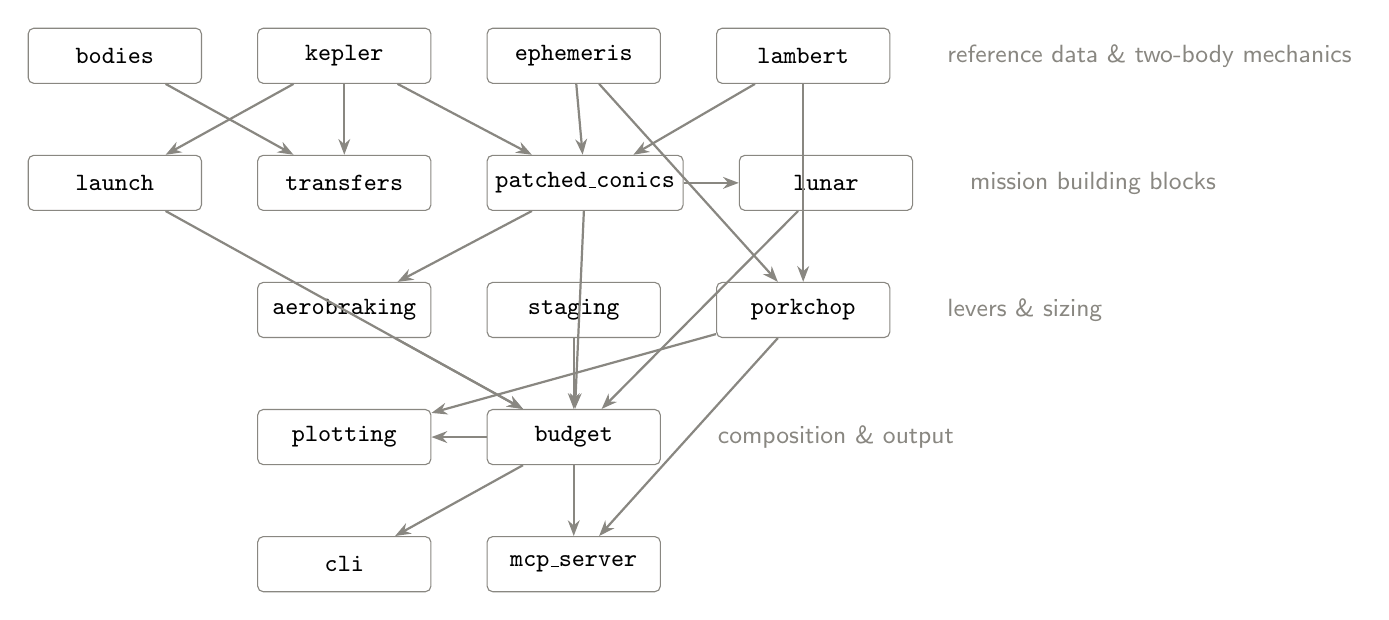
\begin{tikzpicture}[
  box/.style={draw=sfgray,rounded corners=2pt,fill=white,minimum height=7mm,minimum width=22mm,font=\small\ttfamily,inner sep=3pt},
  lay/.style={font=\small\sffamily\color{sfgray},anchor=west},
  arr/.style={-{Stealth[length=2mm]},draw=sfgray,thick},
  node distance=5mm and 7mm]
\node[box] (bodies) {bodies};
\node[box,right=of bodies] (kepler) {kepler};
\node[box,right=of kepler] (eph) {ephemeris};
\node[box,right=of eph] (lam) {lambert};
\node[box,below=9mm of kepler] (tr) {transfers};
\node[box,right=of tr] (pc) {patched\_conics};
\node[box,right=of pc] (lun) {lunar};
\node[box,left=of tr] (launch) {launch};
\node[box,below=9mm of tr] (aero) {aerobraking};
\node[box,right=of aero] (stg) {staging};
\node[box,right=of stg] (pork) {porkchop};
\node[box,below=9mm of stg] (bud) {budget};
\node[box,left=of bud] (plot) {plotting};
\node[box,below=9mm of bud] (mcp) {mcp\_server};
\node[box,left=of mcp] (cli) {cli};
\draw[arr] (bodies) -- (tr); \draw[arr] (kepler) -- (tr); \draw[arr] (kepler) -- (pc); \draw[arr] (eph) -- (pc);
\draw[arr] (lam) -- (pc); \draw[arr] (kepler) -- (launch); \draw[arr] (pc) -- (lun); \draw[arr] (pc) -- (aero);
\draw[arr] (eph) -- (pork); \draw[arr] (lam) -- (pork); \draw[arr] (pc) -- (bud); \draw[arr] (lun) -- (bud);
\draw[arr] (launch) -- (bud); \draw[arr] (aero) -- (bud); \draw[arr] (stg) -- (bud); \draw[arr] (pork) -- (plot);
\draw[arr] (bud) -- (plot); \draw[arr] (bud) -- (mcp); \draw[arr] (bud) -- (cli); \draw[arr] (pork) -- (mcp);
\node[lay] at ([xshift=6mm]lam.east) {reference data \& two-body mechanics};
\node[lay] at ([xshift=6mm]lun.east) {mission building blocks};
\node[lay] at ([xshift=6mm]pork.east) {levers \& sizing};
\node[lay] at ([xshift=6mm]bud.east |- bud) {composition \& output};
\end{tikzpicture}}

\small Pure functions returning dataclasses; km, s, rad internally; degrees for \code{*\_deg} arguments; epochs as ISO strings or JD. 85 tests run in \SI{1}{s}.
\end{frame}

%------------------------------------------------------------------
\begin{frame}{Approach I --- reference data and their accuracy}
\small
\begin{columns}[T]
\begin{column}{0.5\textwidth}
\begin{itemize}
\item $GM$: JPL DE440 (planet-\emph{system} values for outer planets); IAU radii; Laplace SOI $a(m/M)^{2/5}$
\item Planets: JPL \emph{Keplerian Elements for Approximate Positions} --- six elements + secular rates, J2000 ecliptic
\item Moon: truncated Meeus Ch.~47 (32 lon/dist, 20 lat terms), precessed to J2000
\item ``Earth'' = Earth--Moon barycenter unless corrected
\end{itemize}
\end{column}
\begin{column}{0.48\textwidth}
\footnotesize
\begin{tabular}{@{}lccc@{}}\toprule
vs.\ astropy & angle [$''$] & rel.\ dist. & $v$ [m/s] \\\midrule
Inner planets & $<35$ & $<\num{1.5e-4}$ & $<5$ \\
Jupiter & $<340$ & $<\num{4e-4}$ & $<28$ \\
Saturn & $<560$ & $<\num{1.5e-3}$ & $<41$ \\
Uranus/Neptune & $<110$ & $<\num{1e-3}$ & $<16$ \\
Moon & $<40$ & $<\SI{40}{km}$ & -- \\\bottomrule
\end{tabular}
\medskip

Consequence for design: $\vinf$ errors $\sim\SI{1}{m/s}$ at Earth, $\sim\SI{10}{m/s}$ at Saturn --- far below budget margins.
\end{column}
\end{columns}
\end{frame}

%------------------------------------------------------------------
\begin{frame}{Approach II --- Lambert arcs and porkchop maps}
\small
\begin{columns}[T]
\begin{column}{0.46\textwidth}
Universal-variable Lambert (BMW/Curtis):
\[
F(z)=\Big[\tfrac{y}{C}\Big]^{3/2}S+A\sqrt{y}-\sqrt{\mu}\,\Delta t=0
\]
\begin{itemize}
\item $F$ monotonic on the single-rev branch $\Rightarrow$ bracket + Brent: never diverges
\item type I ($<180^\circ$) and type II fall out of the prograde geometry
\item \SI{55}{\micro s} per solve; $110^2$ grid in $\sim$\SI{1}{s}
\item each cell: $C_3$, $\vinf^{arr}$, $\dv_{dep}$, $\dv_{cap}$, DLA
\end{itemize}
Earth$\to$Mars 2026/27 optimum: depart 2026-10-30, 311~d, $C_3=9.2$, $\dv=\SI{5.66}{km/s}$ (300~km parking $\to$ 400~km Mars orbit).
\end{column}
\begin{column}{0.54\textwidth}
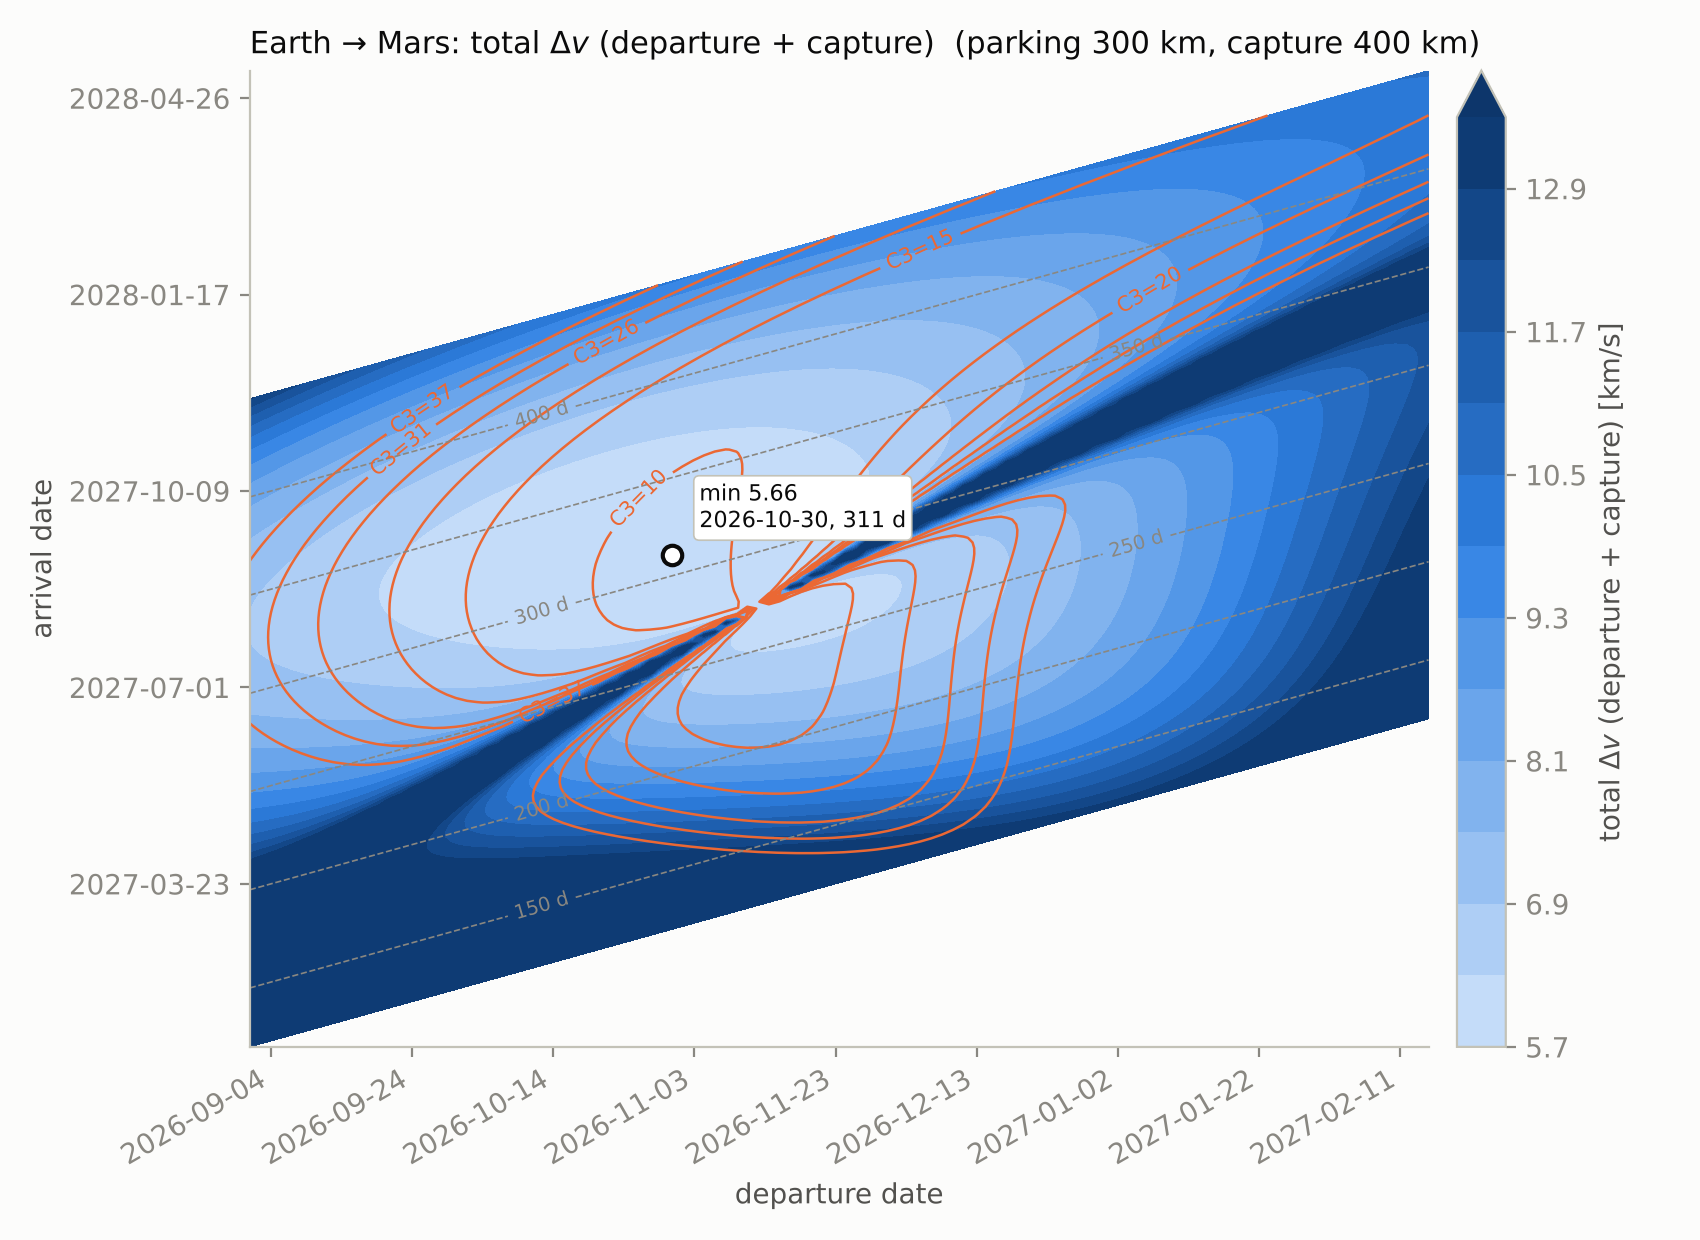
\includegraphics[width=\linewidth]{porkchop_earth_mars_2026_dvtotal}
\end{column}
\end{columns}
\end{frame}

%------------------------------------------------------------------
\begin{frame}{Approach III --- patched conics}
\small
\begin{columns}[T]
\begin{column}{0.54\textwidth}
\textbf{Departure / capture} (tangential periapsis burns)
\[
\dv_{dep}=\sqrt{\vinf^2+\tfrac{2\mu}{r_p}}-\sqrt{\tfrac{\mu}{r_p}},\quad
\dv_{cap}=\sqrt{\vinf^2+\tfrac{2\mu}{r_p}}-v_p^{orbit}
\]
\textbf{Unpowered flyby}
\[
e=1+\frac{r_p\vinf^2}{\mu},\quad \delta=2\arcsin\frac1e,\quad |\dv_{helio}|=2\vinf\sin\frac{\delta}{2}
\]
\textbf{Powered flyby} (MGA model): shared $r_p$ with
$\tfrac12\delta_{in}+\tfrac12\delta_{out}=\angle(\bm\vinf^{in},\bm\vinf^{out})$,
speed mismatch burned at periapsis; infeasible if $r_p<r_{min}$.
\end{column}
\begin{column}{0.44\textwidth}
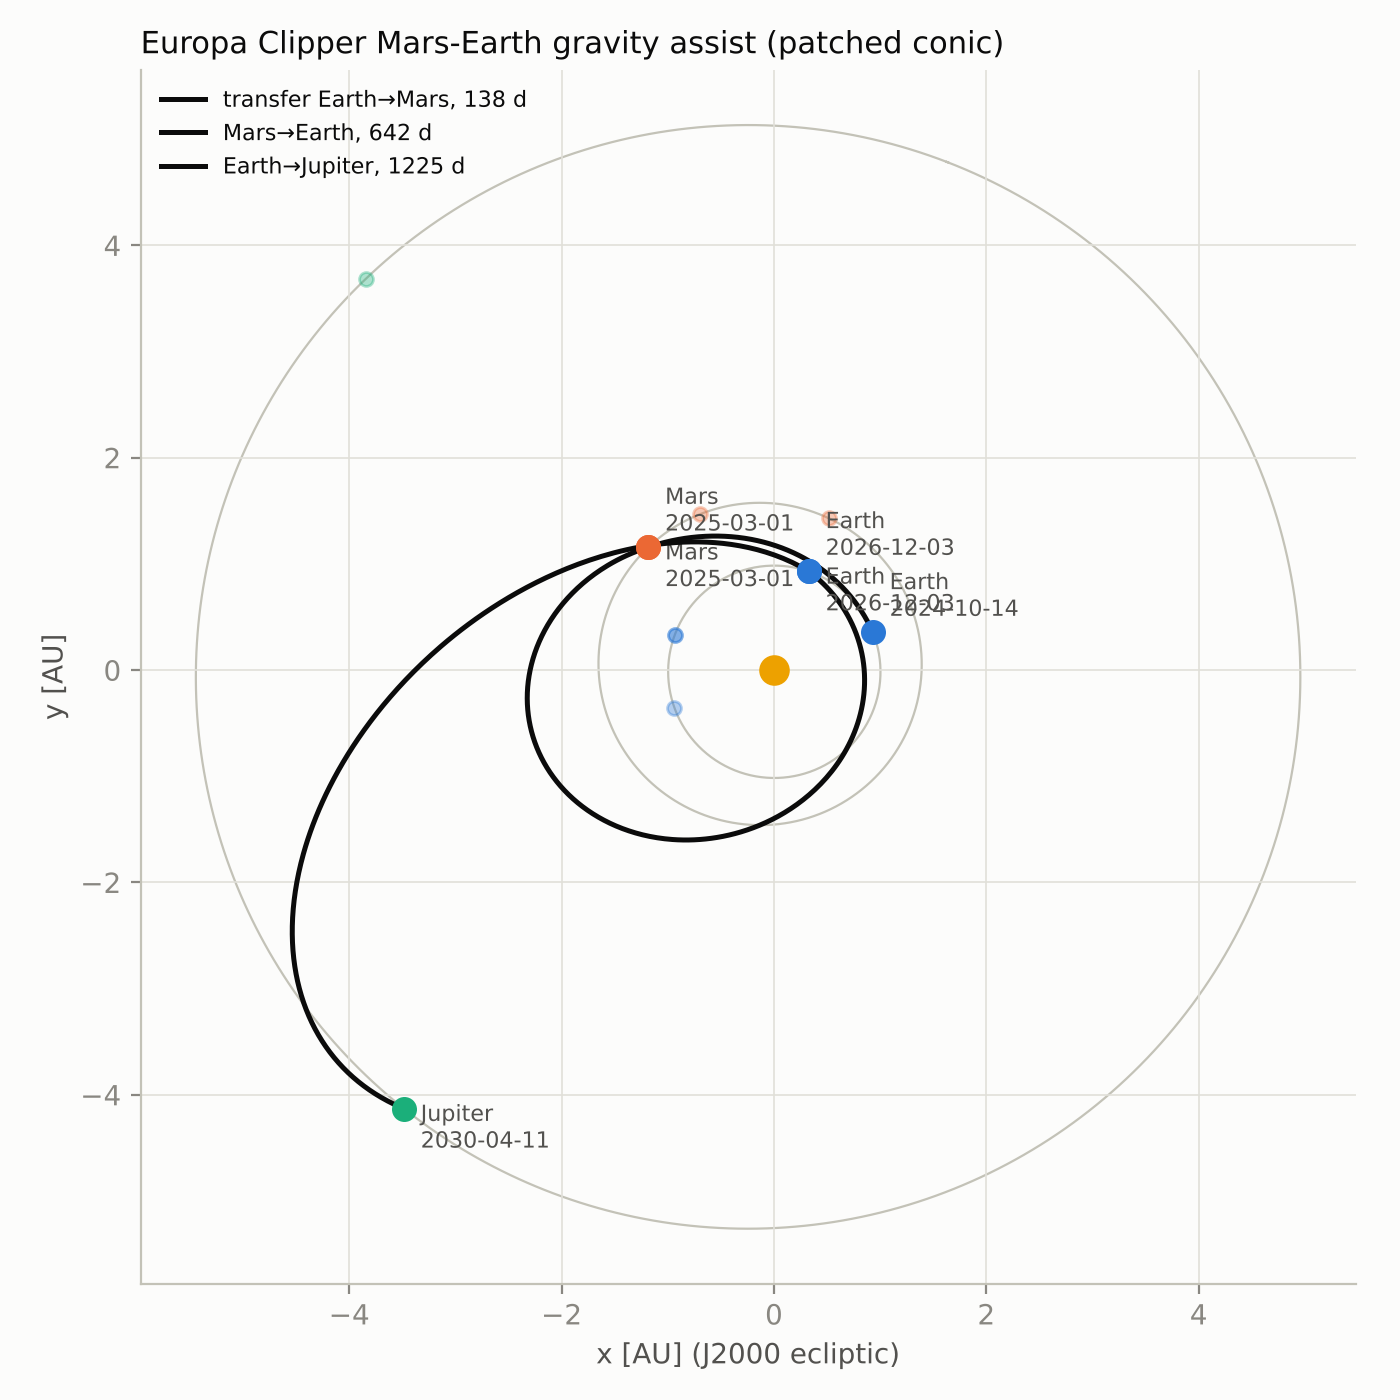
\includegraphics[width=0.9\linewidth]{transfer_europa_clipper_mega}
\scriptsize Europa Clipper dates: $C_3$ 41 vs.\ 77 direct; injection 4.95 vs.\ 6.30~km/s; powered corrections 0.13 + 0.13~km/s at Mars and Earth.
\end{column}
\end{columns}
\end{frame}

%------------------------------------------------------------------
\begin{frame}{Approach IV --- Earth--Moon patched conic (Bate--Mueller--White \S7.4)}
\small
\begin{columns}[T]
\begin{column}{0.52\textwidth}
\begin{itemize}
\item Geocentric ellipse from $(r_0,v_0,\phi_0)$ to the SOI point set by $\lambda_1$
\item $\bm v_2=\bm v_1-\bm v_{Moon}$ $\rightarrow$ selenocentric hyperbola $(e, r_p, v_p)$
\item \textbf{Vector implementation}: sense of motion from $\mathrm{sign}(h_2)$, no trig sign ambiguities (scalar relations reproduced in tests)
\item Adds the \textbf{SOI transit time} (14--18~h) --- essential to compare with flown data
\item Design solver: $\lambda_1$ for given $v_0$ (or $v_0$ for $\lambda_1$) hitting a perilune altitude; prograde and retrograde roots
\end{itemize}
Hohmann estimate: TLI 3.135, LOI 0.82~km/s; 3-day transfer: TLI 3.157, LOI 0.889~km/s.
\end{column}
\begin{column}{0.46\textwidth}
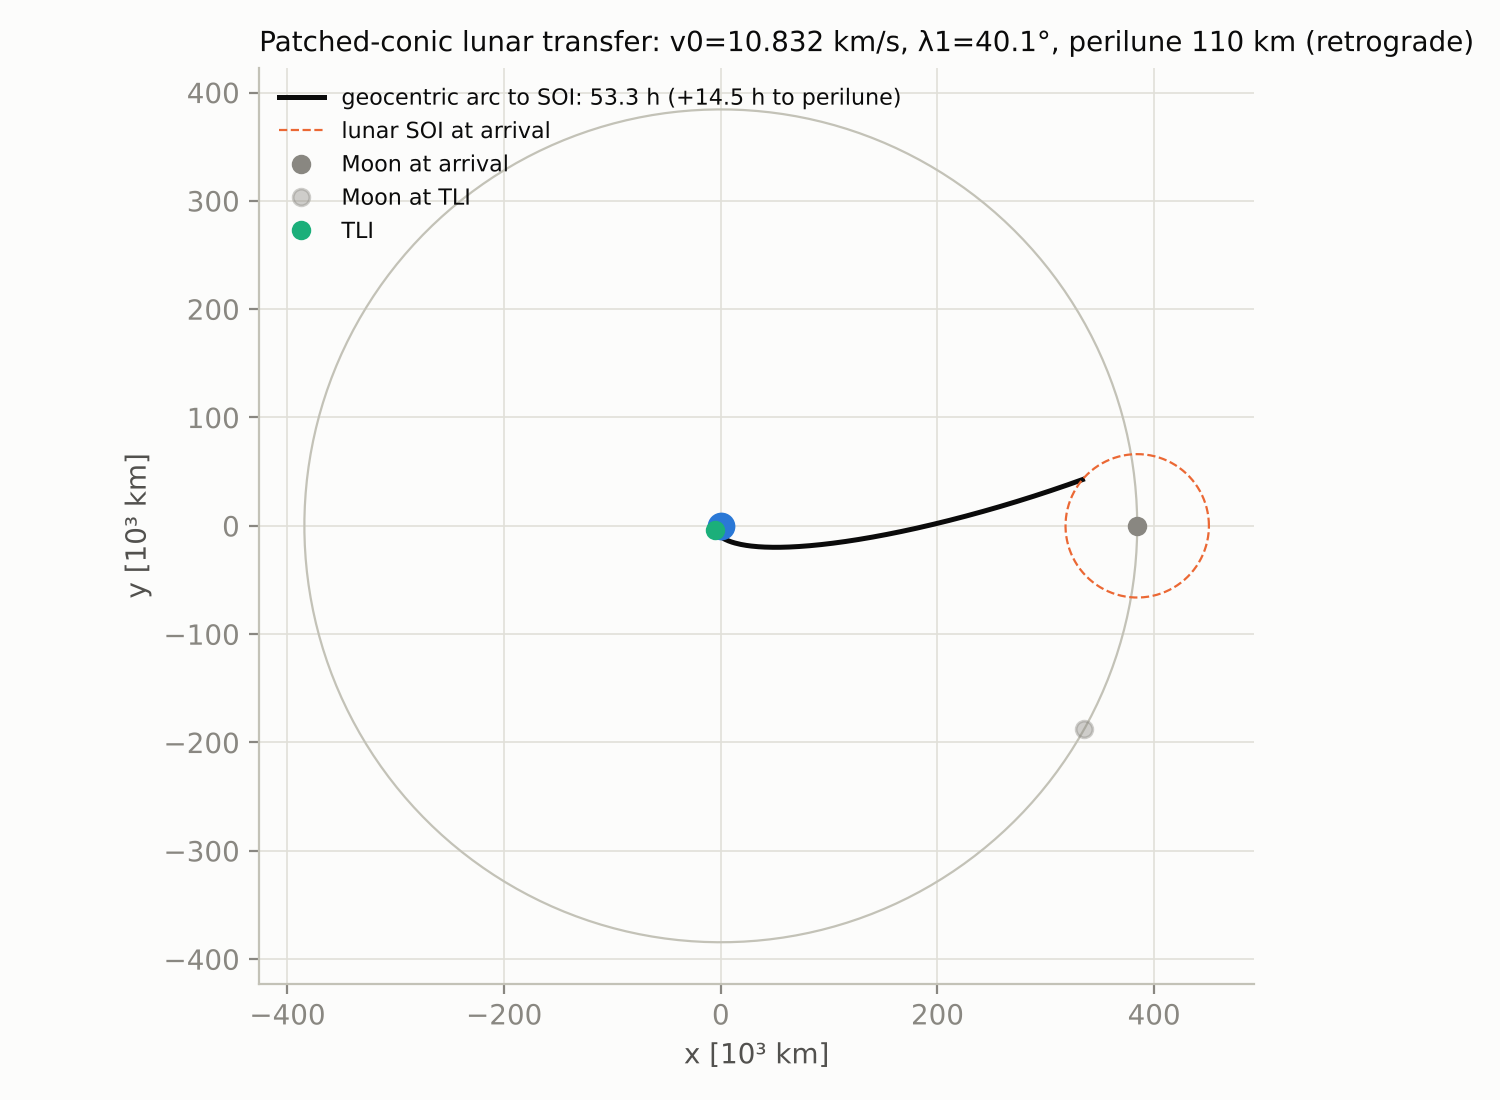
\includegraphics[width=0.95\linewidth]{lunar_patched_conic_apollo11}
\end{column}
\end{columns}
\end{frame}

%------------------------------------------------------------------
\begin{frame}{Approach V --- launch $\dv$ and the aero levers}
\small
\begin{columns}[T]
\begin{column}{0.56\textwidth}
\textbf{Launch}
\[
\dv=|\bm v_{orbit}-\bm v_{site}|+\dv_{grav}+\dv_{drag}+\dv_{steer}
\]
\vspace{-2ex}

with $\bm v_{site}=\omega R\cos\varphi\,\hat{\bm e}_E$ and $\cos i=\cos\varphi\sin Az$. KSC, 300~km, due east: $7.726-0.409+(1.15\ldots2.05)=\SIrange{8.47}{9.37}{km/s}$.

\medskip
\textbf{Aerobraking, per pass} (exponential atmosphere, parabolic $r(t)$ about periapsis)
\[
\dv_{pass}=\frac{\rho_pV_p^2}{2\beta}\sqrt{\frac{2\pi H}{\ddot r_p}},\qquad
\ddot r_p=\frac{V_p^2}{r_p}-\frac{\mu}{r_p^2}
\]
\alert{Dropping $\mu/r_p^2$ (straight-line fly-through) gives the Week-11 slide form, low by $\sqrt{V_p^2/(V_p^2-\mu/r_p)}\to\sqrt2$}; integration confirms the gravity-aware form to 0.2\%.
\end{column}
\begin{column}{0.42\textwidth}
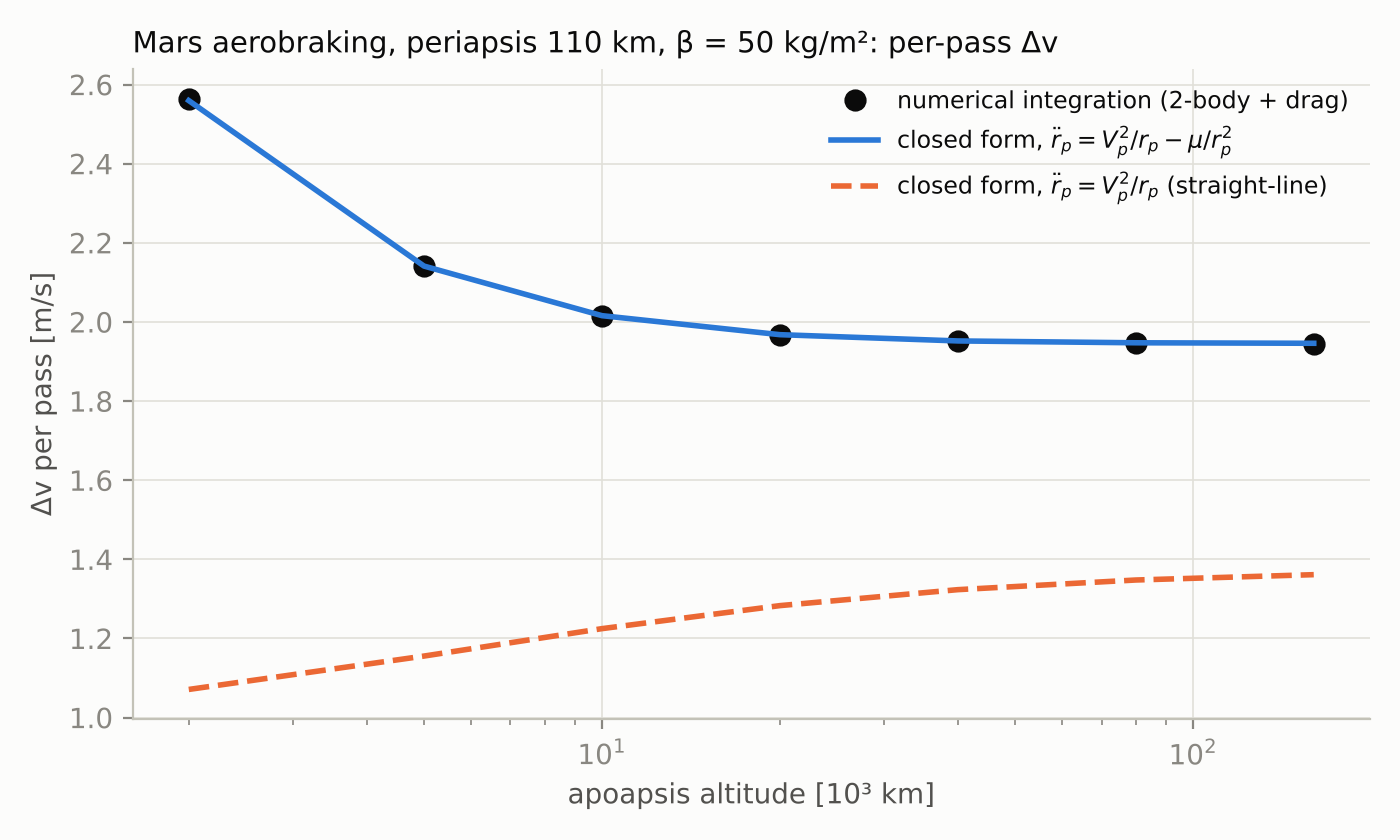
\includegraphics[width=0.9\linewidth]{aerobraking_pass_comparison}
\scriptsize Aerocapture credit at Mars ($\vinf=2.65$): 2.08~km/s replaced by a 0.06~km/s periapsis raise.
\end{column}
\end{columns}
\end{frame}

%------------------------------------------------------------------
\begin{frame}{Approach VI --- rocket equation, staging, budgets}
\small
\begin{columns}[T]
\begin{column}{0.58\textwidth}
Sutton nomenclature: $\zeta=m_p/m_0$, $MR=m_f/m_0$, $\sigma_k=m_{s,k}/(m_{s,k}+m_{p,k})$, $c_k=g_0I_{sp,k}$, $r_k=e^{\dv_k/c_k}$ \; ($\varepsilon$ reserved for area ratio)
\[
\frac{m_0}{m_L}=\prod_k\frac{r_k(1-\sigma_k)}{1-r_k\sigma_k},\qquad
I_{sp}^{req}=\frac{\dv}{g_0\,\ln[1/(1-\zeta)]}
\]
Optimal split for fixed $\sum\dv_k$ (one scalar root in $\lambda$):
\[
r_k=\frac{\lambda c_k-1}{\lambda c_k\sigma_k},\qquad \sum_k c_k\ln r_k=\dv_{tot}
\]
\end{column}
\begin{column}{0.40\textwidth}
\begin{block}{\code{DeltaVBudget}}
ordered legs with nominal/low/high, kind (propulsive / aero / margin), optional stage $I_{sp}$
\begin{itemize}
\item composers: dated interplanetary (launch, injection, flybys, capture or aerocapture, landing, margin); lunar (TLI, LOI, descent, ascent, TEI)
\item backward propellant sizing; $\zeta$ and required $I_{sp}$ --- the hand-off to engine design
\end{itemize}
\end{block}
\end{column}
\end{columns}
\end{frame}

%------------------------------------------------------------------
\begin{frame}{Validation --- textbook, independent models, flown missions}
\footnotesize
\begin{tabular}{p{0.44\textwidth}p{0.52\textwidth}}\toprule
Lambert, Curtis Ex.~5.2; 20 closure geometries & $\bm v_1,\bm v_2$ to \SI{1e-4}{km/s}; closes to \SI{1e-8}{km} \\
Earth$\to$Mars Hohmann (Curtis Ex.~8.4--8.6) & $\vinf$ 2.943/2.648, $\dv$ 3.590~km/s, phase $44.3^\circ$, synodic 779.9~d \\
LEO$\to$GEO; $+28.5^\circ$ plane change & 3.893~km/s; 4.23~km/s \\
\textbf{Mars 2020} actual dates & path \SI{470.9}{Mkm} vs.\ $\approx$\SI{471}{Mkm} (JPL); $C_3$ 14.5; $\vinf^{arr}$ 2.55~km/s \\
\textbf{Voyager 2} E--J--S dates & Jupiter turn $97^\circ$; $r_p$ 620,000 vs.\ $\approx$570,000~km; powered fix 0.05~km/s; $C_3$ 105 \\
\textbf{Apollo 11} published TLI state & TLI$\to$perilune 68--73~h vs.\ 73.0~h; LOI 0.89--0.92 vs.\ 0.891~km/s \\
Aerobraking pass vs.\ integration & 1.952 vs.\ 1.951~m/s \\
Ephemeris vs.\ astropy; Mars oppositions & table on slide 5; longitudes agree $<1.5^\circ$ \\
Staging identities, optimal split & exact \\\bottomrule
\end{tabular}
\medskip

\small Lecture point from Apollo 11: the two published TLI rows differ by \SI{0.04}{km^2/s^2} in energy, and lunar TOF moves $\sim$\SI{5}{h} per \SI{0.1}{km^2/s^2} --- the result is as good as the altitude datum.
\end{frame}

%------------------------------------------------------------------
\begin{frame}{Utility --- numbers for Week 10}
\small
\begin{columns}[T]
\begin{column}{0.52\textwidth}
\footnotesize
\begin{tabular}{@{}p{0.5\linewidth}p{0.2\linewidth}p{0.25\linewidth}@{}}\toprule
Lever (Mars $\vinf=2.65$~km/s) & without & with \\\midrule
Aerocapture, 400~km orbit & 2.08~km/s & 0.06~km/s \\
Aerobraking 110$\times$40,000$\to$400~km & 2.08~km/s & 0.92~km/s, 152~d \\
Mars--Earth assist to Jupiter & $C_3$ 77, 2.7~yr & $C_3$ 41, 5.5~yr \\
KSC credit, east vs.\ polar & 0.41~km/s & $-0.01$~km/s \\\bottomrule
\end{tabular}
\medskip

\begin{itemize}
\item Earth--Mars phase angle on 11/12: $56^\circ$ vs.\ $44.3^\circ$ Hohmann requirement
\item Type II (311~d, 5.66~km/s) vs.\ type I (260~d, 6.02~km/s) in this window
\item Next windows: 2028-11, 2030-12/2031-02, 2033-03/04 (type II / type I pairs)
\end{itemize}
\end{column}
\begin{column}{0.46\textwidth}
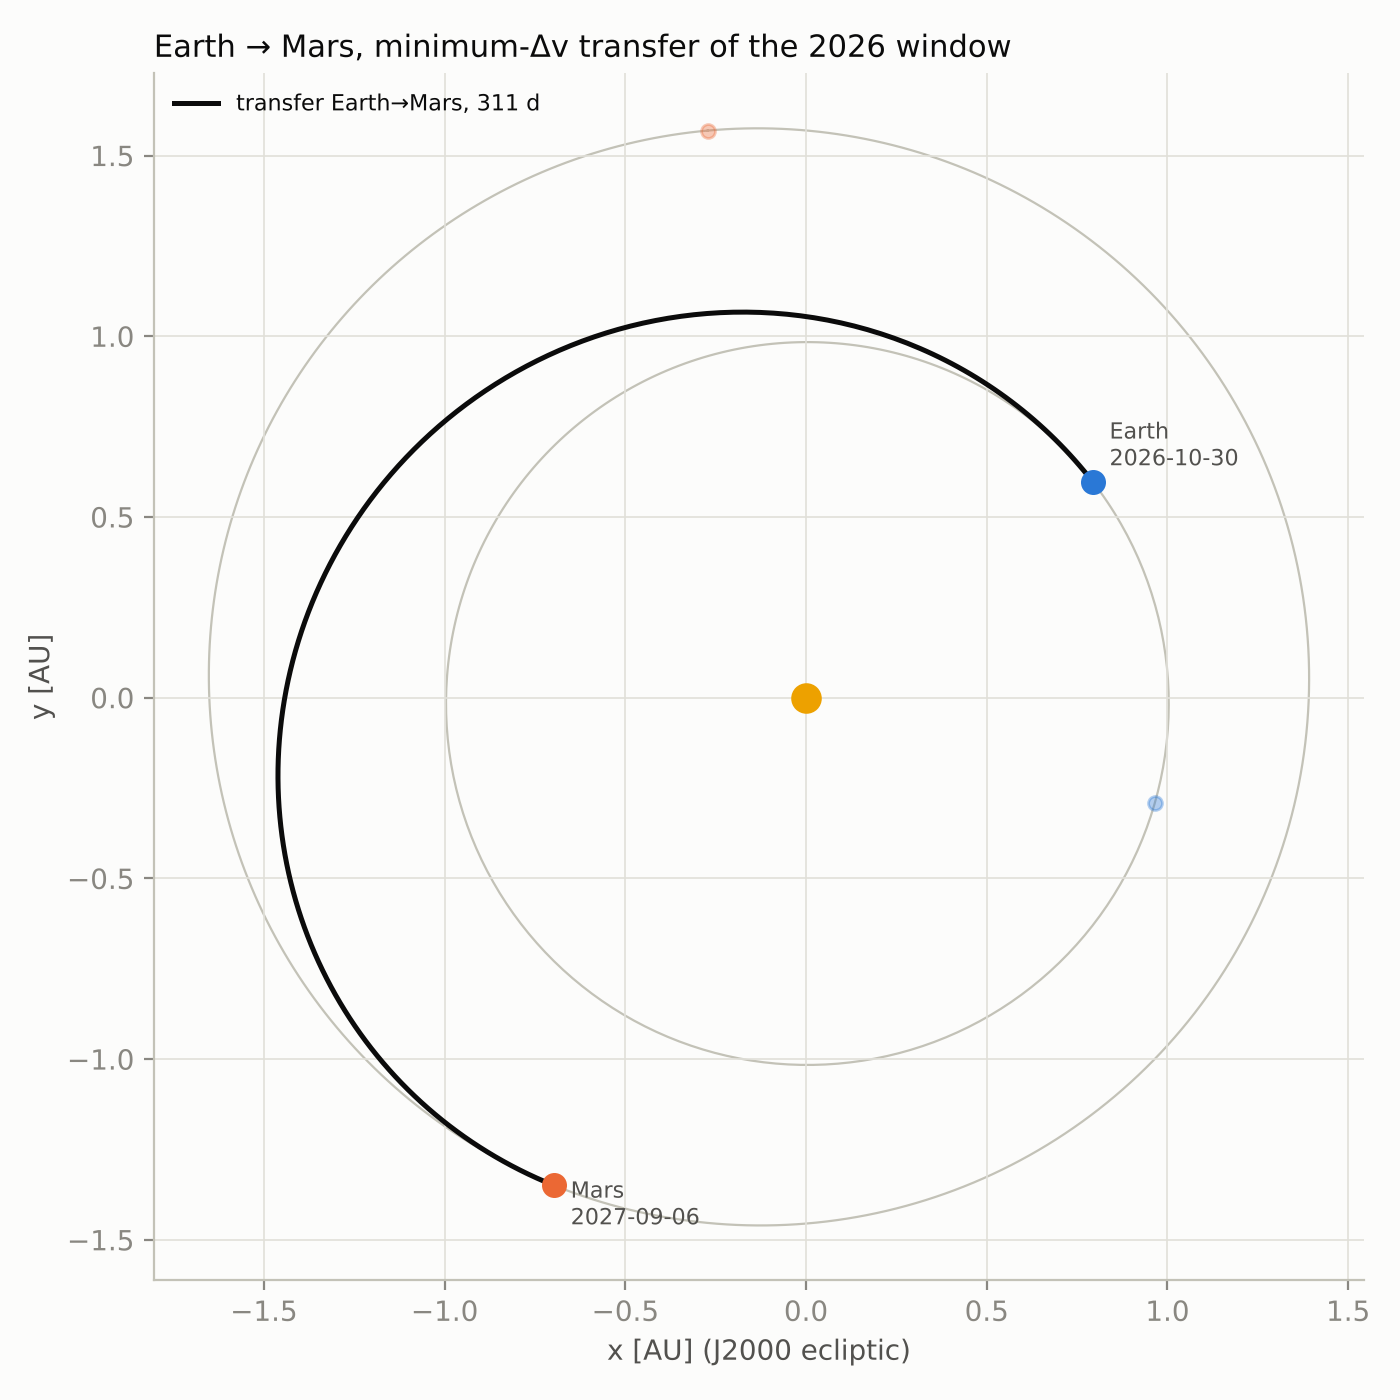
\includegraphics[width=\linewidth]{transfer_earth_mars_2026}
\end{column}
\end{columns}
\end{frame}

%------------------------------------------------------------------
\begin{frame}{Utility --- HW 1 reference chain (steps 1--4 end to end)}
\small
\begin{columns}[T]
\begin{column}{0.5\textwidth}
Mars orbiter, 2026 window, KSC:
\begin{enumerate}
\item launch band 8.47--9.37~km/s
\item dated legs at the porkchop optimum
\item budgets: post-launch $\dv$ \textbf{6.39} (propulsive) vs.\ \textbf{4.31}~km/s (aerocapture)
\item required $I_{sp}$ at $\zeta=0.7$: 541~s vs.\ 365~s
\item 1000~kg final mass, 320-s engine $\rightarrow$ 7,653~kg injected
\item two-stage launcher ($I_{sp}$ 300/450, $\sigma$ 0.07/0.10) for 12.5~km/s: gross 695~t, optimal split 4.8/7.7~km/s
\end{enumerate}
\small Teams swap mission, dates and engines; the \code{DeltaVBudget} feeds the Week 11--12 thermochemistry and engine modules.
\end{column}
\begin{column}{0.48\textwidth}
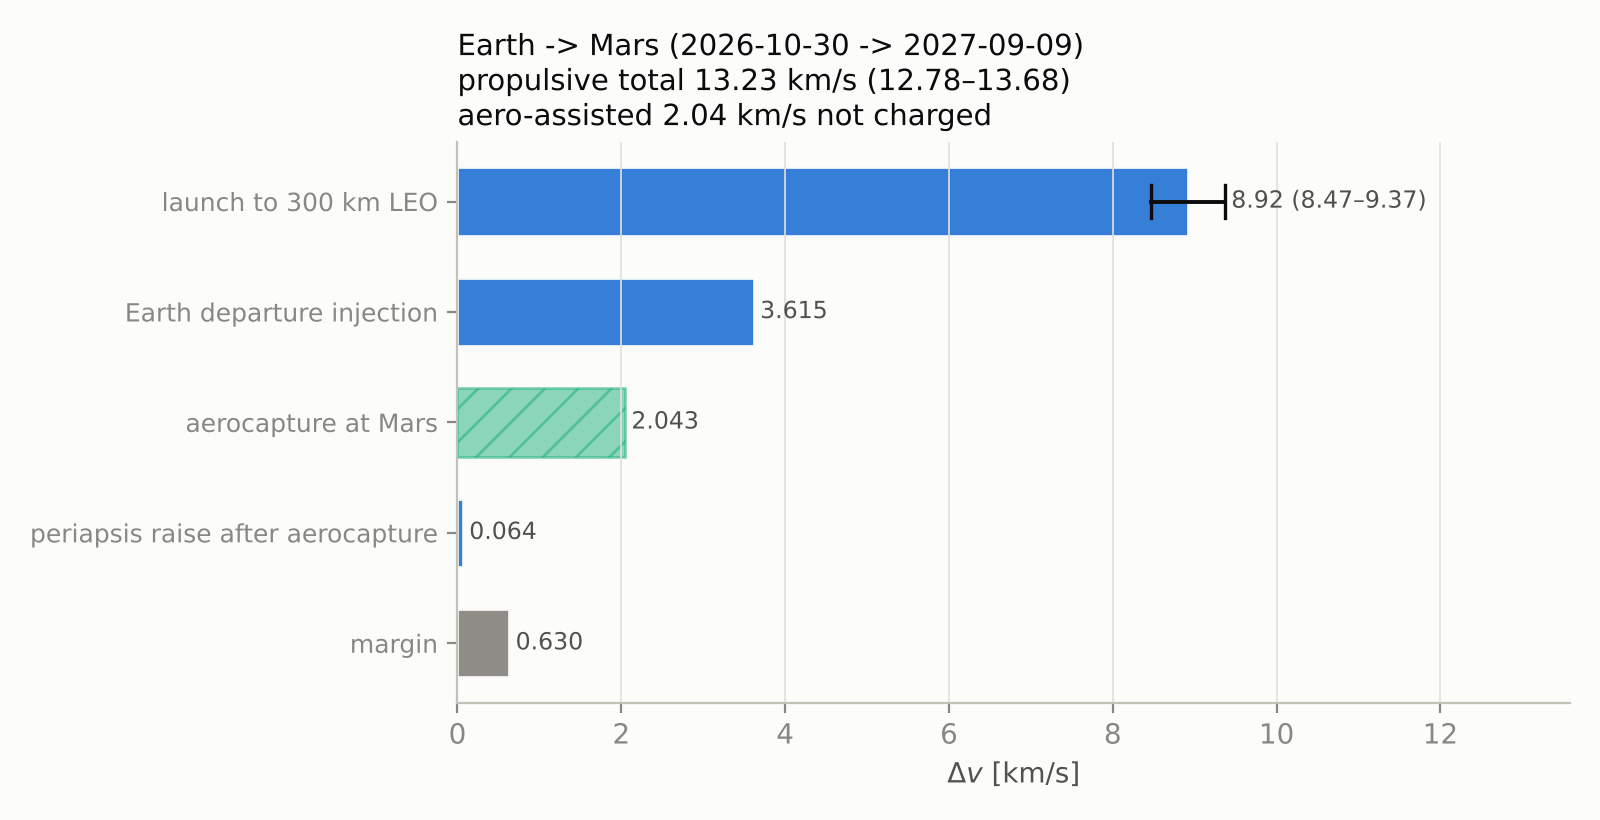
\includegraphics[width=\linewidth]{hw1_budget_aero}
\end{column}
\end{columns}
\end{frame}

%------------------------------------------------------------------
\begin{frame}{Limitations I --- physics}
\begin{itemize}
\item \textbf{Patched conics}: no third-body gravity on a conic, sharp SOI. Few-\% error in planetocentric burns for planetary missions; hours of TOF and tens of m/s of LOI for the Moon (Apollo 11: 0--7\%).
\item \textbf{Impulsive burns}: finite-burn losses of low-$T/W$ stages not charged; launch losses are a user band, not a trajectory.
\item \textbf{Ephemeris}: arcsec--arcmin mean elements; Earth = EM barycenter by default. Fine for $\dv$, not for targeting.
\item \textbf{Circular assumptions}: Moon orbit circular at 384,400~km (perigee--apogee $\pm$21,000~km $\Rightarrow$ $\pm$10~m/s TLI, hours of TOF); quick estimates use circular coplanar planets.
\item \textbf{Plane/DLA}: 3-D legs, but no plane-change penalty for high-DLA departures or parking-orbit incompatibility; DLA reported only.
\item \textbf{Lambert}: single revolution; $180^\circ$ transfers undefined (NaN ridge).
\item \textbf{Powered flyby}: shared-periapsis tangential-burn model is a lower bound; flyby dates are inputs, not optimized.
\end{itemize}
\end{frame}

%------------------------------------------------------------------
\begin{frame}{Limitations II --- scope}
\begin{columns}[T]
\begin{column}{0.5\textwidth}
\textbf{Aero-assist}
\begin{itemize}
\item aerocapture charged as a $\dv$ credit only: no corridor, heating, g-load, TPS mass, guidance
\item single-scale-height atmosphere fitted to 90--150~km; constant $\beta$; Mars density varies $\times2$ $\Rightarrow$ pass count and duration do too
\end{itemize}
\textbf{Staging}
\begin{itemize}
\item $\sigma$ is an input; no $T/W$, tank or residual models; $\sigma_k$ independent of stage size
\end{itemize}
\end{column}
\begin{column}{0.48\textwidth}
\textbf{Reference values, not computed}
\begin{itemize}
\item lunar descent/ascent 2.07/1.86~km/s (Apollo LM); Mars landing $\dv$ user-supplied
\end{itemize}
\textbf{Not covered}
\begin{itemize}
\item low-thrust / electric trajectories
\item launch-vehicle performance curves ($C_3$ vs.\ payload)
\item navigation and statistical $\dv$, environments, operations
\end{itemize}
\end{column}
\end{columns}
\end{frame}

%------------------------------------------------------------------
\begin{frame}[fragile]{Next steps and how to run it}
\begin{columns}[T]
\begin{column}{0.5\textwidth}
\textbf{Planned (priority order)}
\begin{enumerate}
\item low-thrust legs: Edelbaum $\dv$, power-limited sizing (HW~3b, EP teams)
\item DE440 option + perturbed propagator to quantify patched-conic error on request
\item multi-revolution Lambert
\item launch-vehicle performance curves
\item coupling to the ascent-trajectory optimizer (computed launch band)
\end{enumerate}
\end{column}
\begin{column}{0.48\textwidth}
\begin{lstlisting}
pip install -e ".[dev,mcp]"      # repo root
pytest tests/mission_analysis    # 85 tests

from modern_aerospace_propulsion.mission_analysis import *
pc = porkchop("Earth","Mars","2026-09-01","2027-02-15",120,450)
print(pc.summary())
b, m = interplanetary_budget("Earth","Mars",
        "2026-10-30","2027-09-06", aerocapture=True)
print(b.table()); b.size_propellant(1000, 320)

sfmission lunar --tof 72 --plot lunar.png
sfmission-mcp     # {"mcpServers":{"sfmission":
                  #   {"command":"sfmission-mcp"}}}
\end{lstlisting}
\small Code, tests, examples, figures, report and these slides: \code{Week 10 - Mission Analysis/} in the course repository.
\end{column}
\end{columns}
\end{frame}

\end{document}
